\section{Huffmankoding}\label{huffman}
Huffmankoding er en måte å kode informasjon på (her tekst) på en måte der vi ikke mister noe informasjon (\textit{lossless}). Den forutsetter at vi har tilgang på teksten før vi lager en kode. Huffmankoding går ut på å se på frekvensen til tegnene som forekommer, og gi kort kode til de tegnene som forekommer ofte, og lang kode til de som forekommer sjelden. Når vi velger disse kodene er det viktig at vi beholder det vi kaller \say{prefiksegenskapen:} Ingen koder er et prefiks av noen andre. Kodealfabetet $ \{9, 55\} $ har prefiksegenskapen, men $ \{9, 5, 59, 55\} $ har ikke, siden 5 er prefiks i $ 55 $ og $ 59 $. Måten Huffmankoding beholder denne egenskapen blir fort tydelig når vi ser på algoritmen. 

\begin{theorem} Algoritme for Huffman-koding

\begin{enumerate}
	\item Lag frekvenstabell for alle tegn som forekommer i teksten.
	\item Sett alle frekvensene inn i en heap $ P $
	\item Mens $P$ har mer enn ett element:
	\begin{itemize}
		\item Ta ut de to minste nodene fra $P$.	
		\item Slå sammen nodene, og summer frekvensene.
		\item Legg den nye noden inn i $P$.	
	\end{itemize}
	\item Vi leser koden til et tegn ved å følge stien fra rotnoden ned til tegnets løvnode. Vi får en `0' når vi går til venstre, og en `1' når vi går til høyre. (Dette fungerer selvfølgelig ved å gjøre motsatt, så lenge man er konsekvent.) 
\end{enumerate}
\end{theorem}

\noindent \textbf{Merk:} En tekst kan ha flere gyldige Huffman-trær, og dermed flere gyldige Huffman-kodinger. 

~\\

\noindent Algoritmen burde bli klar når vi ser på et eksempel.
\newpage
\begin{example}
	Anta at vi har en tekst ``BACADAEAFABBAAAGAH''. Vi setter opp en frekvenstabell for bokstavene i koden.
	\begin{center}
		\begin{tabular}{c c c}
			Tegn & Frekvens \\
			\hline
			A & 9\\
			B & 3\\
			C & 1\\
			D & 1\\
			E & 1\\
			F & 1\\
			G & 1\\
			H & 1
		\end{tabular}
	\end{center}
	Vi ser at vi kan parvis slå sammen to og to av nodene som har vekt 1: Vi slår sammen C og D, E og F, og G og H. Nå har (CD), (EF) og (GH) alle vekt 2. Vi slår så sammen B og (CD) til en node (B, CD) med vekt 5, og vi slår sammen (EF) og (GH) til en node (EF, GH) med vekt 4. Vi slår så igjen sammen (B, CD) og (EF, GH) slik at de får en foreldrenode med vekt 9. Til slutt slår vi sammen denne med noden A. Det resulterende treet er:
	
	\begin{figure}[H]
		\centering
		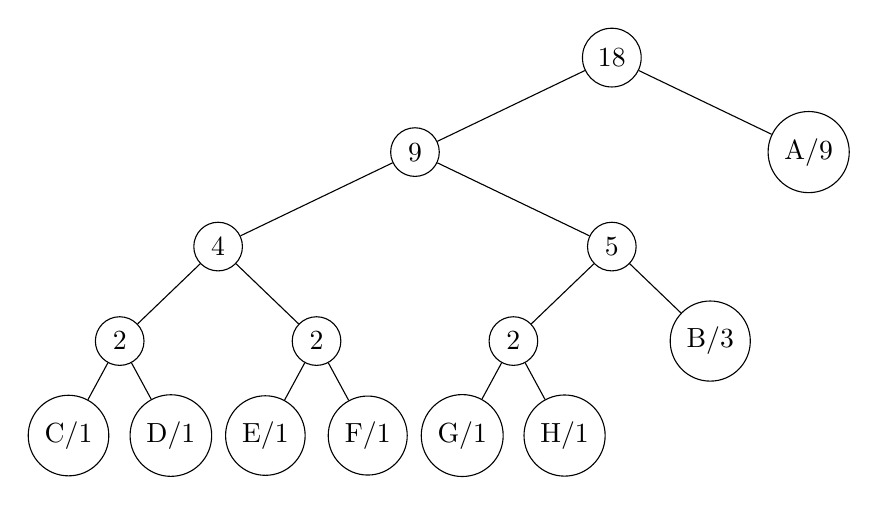
\begin{tikzpicture}[level distance=1.2cm,
		level 1/.style={sibling distance=5cm},
		level 2/.style={sibling distance=5cm},
		level 3/.style={sibling distance=4cm},
		level 3/.style={sibling distance=2.5cm},
		level 4/.style={sibling distance=1.3cm}
		]
		\tikzstyle{every node}=[circle,draw]
		
		\node {18}
		child {
			node {9} 
			child {
				node {4}
				child { node {2}
					child {node {C/1}}
					child {node {D/1}}}
				child { node {2}
					child {node {E/1}}
					child {node {F/1}}}
			}
			child {
				node {5}
				child { node {2}
					child {node {G/1}}
					child {node {H/1}}}
				child { node {B/3}
				}
			}
		}
		child {
			node {A/9}
		}
		;
		\end{tikzpicture}
	\end{figure}
	
	Hvis vi nå følger regelen fra algoritmen om å skrive `0' når vi går venstre og 1 når vi går høyre får vi kodene:
	\begin{center}
		\begin{tabular}{c c c}
			Tegn & Frekvens & Kode \\
			\hline
			A & 9 & 1\\
			B & 3 & 011\\
			C & 1 & 0000\\
			D & 1 & 0001\\
			E & 1 & 0010\\
			F & 1 & 0011\\
			G & 1 & 0100\\
			H & 1 & 0101
		\end{tabular}
	\end{center}
	Vi kan lett sjekke at prefiksegenskapen er intakt, og teksten ``BACADAEAFABBAAAGAH'' får koden
	\begin{center}
		\mono{011100001000110010100111011011111010010101}
	\end{center}
	som er $ 42 $ bits lang. Dette er åpenbart mye kortere enn standard enkoding. Hvis vi for eksempel hadde brukt ASCII-enkoding, der hvert tegn har en $ 7 $-bits kode, hadde vi hatt en kode med $7\cdot18 = 126$ bits.
\end{example}